\section{Orientation Gauge and Affine Reflection}
\label{sec:orientation_gauge}

\paragraph{Orientation representative gauge.}
For qubit mean-force parametrisations with longitudinal dressing scalar \(\Sigma_z\), define
\begin{equation}
  \mathcal{G}: \Sigma_z \mapsto -\Sigma_z.
\end{equation}
This is a representative-level \(Z_2\) choice of eigenaxis orientation.

\begin{definition}[Effective-temperature representative]
\label{def:beta_eff}
Let
\begin{equation}
  a := \frac{\beta\omega_q}{2}, \qquad
  u := \gamma(\chi)\,U,
  \qquad \Theta := \operatorname{arctanh}(u)-a,
\end{equation}
with \(|u|<1\). Define the effective-temperature representative
\begin{equation}
  \beff := -\frac{2}{\omega_q}\Theta
  = \beta - \delta\beta,
  \qquad
  \delta\beta:=\frac{2}{\omega_q}\operatorname{arctanh}(u).
\end{equation}
Under \(\mathcal{G}\), \(U\mapsto -U\), hence \(u\mapsto -u\).
\end{definition}

\begin{lemma}[Affine reflection]
\label{lem:affine_reflection}
Under the orientation-gauge map \(\mathcal{G}\),
\begin{equation}
  \beff' = 2\beta - \beff.
\end{equation}
\end{lemma}
\begin{proof}
Since \(u\mapsto -u\), one has
\begin{equation}
  \delta\beta'=\frac{2}{\omega_q}\operatorname{arctanh}(-u)=-\delta\beta.
\end{equation}
Therefore
\begin{equation}
  \beff'=\beta-\delta\beta'
  =\beta+\delta\beta
  =2\beta-(\beta-\delta\beta)
  =2\beta-\beff.
\end{equation}
\end{proof}

\begin{lemma}[Even/odd observable split]
\label{lem:even_odd_split}
Let \(O_{\mathrm{rad}}=F(\chi)\) with no explicit dependence on \(u\). Then
\begin{equation}
  O_{\mathrm{rad}}' = O_{\mathrm{rad}}
  \quad \text{under } \mathcal{G}.
\end{equation}
If \(O_{\mathrm{odd}}=H(\chi,u)\) with \(H(\chi,-u)=-H(\chi,u)\), then
\begin{equation}
  O_{\mathrm{odd}}'=-O_{\mathrm{odd}}.
\end{equation}
For longitudinal thermal representatives, the transformation is affine through
Lemma~\ref{lem:affine_reflection}, not generally a sign flip.
\end{lemma}
\begin{proof}
Gauge action leaves \(\chi\) invariant and flips \(u\). The stated parity properties follow by direct
substitution into \(F\) and \(H\). The affine law for \(\beff\) was proved above.
\end{proof}

\begin{figure}[tbp]
  \centering
  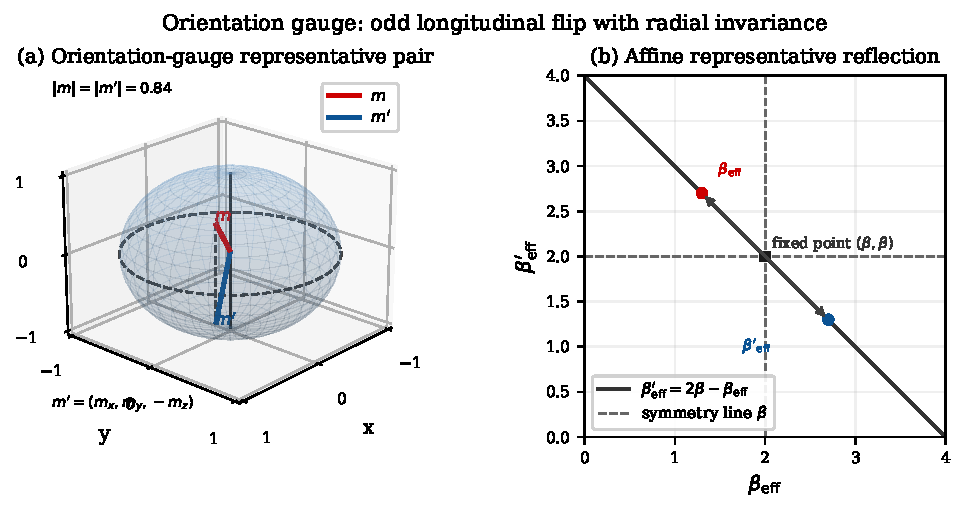
\includegraphics[width=\columnwidth]{../figures/hmf_orientation_gauge_bloch.pdf}
  \caption{
  Geometric action of the orientation gauge.
  \textbf{(a)} Bloch-sphere representative pair \(m\) and \(m'=(m_x,m_y,-m_z)\), connected by the
  dashed longitudinal segment: radius is unchanged (\(|m|=|m'|\)) while the oriented longitudinal
  component flips.
  \textbf{(b)} Affine representative map for effective temperature,
  \(\beta_{\mathrm{eff}}'=2\beta-\beta_{\mathrm{eff}}\), shown as reflection about the fixed point
  \((\beta,\beta)\) and symmetry axes at \(\beta\).
  }
  \label{fig:orientation_gauge_bloch}
\end{figure}

\paragraph{Implementation note.}
Figure~\ref{fig:orientation_gauge_bloch} is generated by
\path{paper_dual_hmf/validation/make_orientation_gauge_bloch_figure.py}.
